\section{Methoden}
	
	Dieser Abschnitt befasst sich mit dem Aufbau des Versuches und den dabei auftretenden Unsicherheiten.
	
	\subsection{Aufbau}	
		
		\begin{figure}[ht]
			\centering
			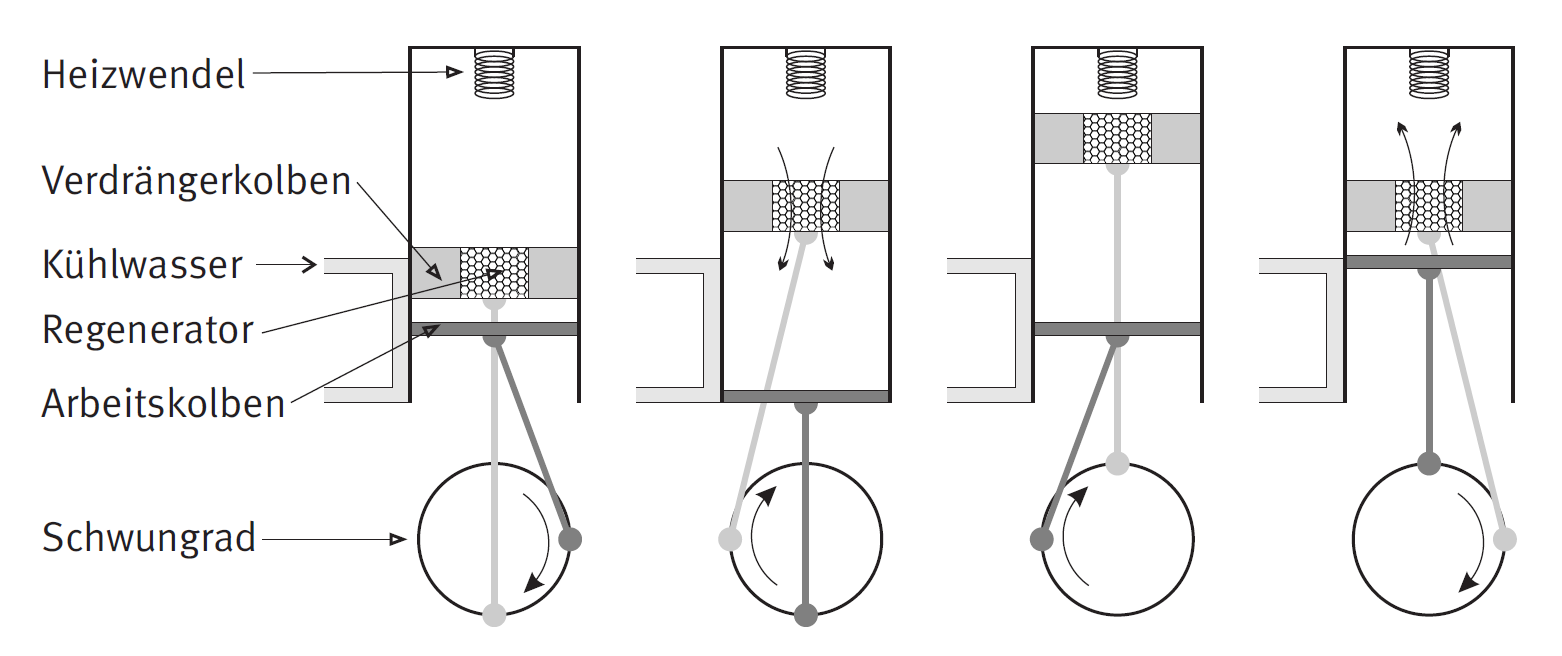
\includegraphics[width=\textwidth]{Aufbau.png}
			\caption{Aufbau des Versuches.\cite{WWU}}
			\label{fig:Aufbau}	
		\end{figure
		Aufbaubeschreibung
				
	\subsection{Unsicherheiten}
	
		Jegliche Unsicherheiten werden nach GUM bestimmt und berechnet\footnote{Die Gleichungen dazu finden sich im Anhang unter \ref{fig:GUM_combine}, \ref{fig:GUM_formula}.}.
		Für die Unsicherheitsrechnungen wurde die Python Bibliothek "uncertainties" herangezogen, welche den Richtlinien des GUM folgt.
	
		Für digitale Messungen wird eine Unsicherheit von $u(X) = \frac{\Delta X}{\sqrt{3}}$ angenommen, bei analogen eine von $u(X) = \frac{\Delta X}{\sqrt{6}}$.
		
		\begin{itemize}
			\item hier konkrete Unsicherheiten beim Messen
		\end{itemize}
		
\section{Durchführung und Datenanalyse}
		
	
\section{Diskussion}
	
	